\documentclass[UTF8]{ctexart}

%固定图片位置
\usepackage{float}

%插入超链接
\usepackage{url}

\usepackage{tikz,mathpazo}
\usetikzlibrary{shapes.geometric, arrows}
\usetikzlibrary{calc}

%\usepackage[affil-it]{authblk}

\usepackage{listings}
%插入代码的配置
\definecolor{CPPLight}  {HTML} {686868}
\definecolor{CPPSteel}  {HTML} {888888}
\definecolor{CPPDark}   {HTML} {262626}
\definecolor{CPPBlue}   {HTML} {4172A3}
\definecolor{CPPGreen}  {HTML} {487818}
\definecolor{CPPBrown}  {HTML} {A07040}
\definecolor{CPPRed}    {HTML} {AD4D3A}
\definecolor{CPPViolet} {HTML} {7040A0}
\definecolor{CPPGray}  {HTML} {B8B8B8}
\lstset{
	language=Python,                                     % 设置语言
    columns=fixed,    
    breaklines = true,   
    basicstyle=\small ,
    numbers=left,                                        % 在左侧显示行号
    %frame=none,                                          % 不显示背景边框
    backgroundcolor=\color[RGB]{245,245,244},            % 设定背景颜色
    keywordstyle=\color[RGB]{40,40,255},                 % 设定关键字颜色
    numberstyle=\tiny\color{darkgray},           % 设定行号格式
    %commentstyle=\it\color[RGB]{0,96,96},                % 设置代码注释的格式
    stringstyle=\rmfamily\slshape\color[RGB]{128,0,0},   % 设置字符串格式
    showstringspaces=false,                              % 不显示字符串中的空格                           
    %morekeywords={True,alignas,continute,friend,register,true,alignof,decltype,goto,
    %reinterpret_cast,try,asm,defult,if,return,typedef,auto,delete,inline,short,
    %typeid,bool,do,int,signed,typename,break,double,long,sizeof,union,case,
    %dynamic_cast,mutable,static,unsigned,catch,else,namespace,static_assert,using,
    %char,enum,new,static_cast,virtual,char16_t,char32_t,explict,noexcept,struct,
    %void,export,nullptr,switch,volatile,class,extern,operator,template,wchar_t,
    %const,false,private,this,while,constexpr,float,protected,thread_local,
    %const_cast,for,public,throw,std,rand},
    emph={access,and,break,class,continue,def,del,elif ,else,%
	except,exec,finally,for,from,global,if,import,in,i s,%
	lambda,not,or,pass,print,raise,return,try,while},
    emphstyle=\color{CPPViolet}, 
    emph={[2]True, False, None, self},
	emphstyle=[2]\color{green},
	emph={[3]from, import, as},
	emphstyle=[3]\color{blue},
	upquote=true,
	morecomment=[s]{"""}{"""},
	commentstyle=\color{orange}\slshape,
	emph={[4]1, 2, 3, 4, 5, 6, 7, 8, 9, 0},
	emphstyle=[4]\color{red},
	emph={[5]numpy, np, plt},
	emphstyle=[5]\color{red},
	literate=*{:}{{\textcolor{blue}:}}{1}%
	{=}{{\textcolor{blue}=}}{1}%
	{-}{{\textcolor{blue}-}}{1}%
	{+}{{\textcolor{blue}+}}{1}%
	{*}{{\textcolor{blue}*}}{1}%
	{!}{{\textcolor{blue}!}}{1}%
	{(}{{\textcolor{blue}(}}{1}%
	{)}{{\textcolor{blue})}}{1}%
	{[}{{\textcolor{blue}[}}{1}%
	{]}{{\textcolor{blue}]}}{1}%
	{<}{{\textcolor{blue}<}}{1}%
	{>}{{\textcolor{blue}>}}{1},%
	framexleftmargin=0.1mm, framextopmargin=0.1mm, frame=shadowbox, rulesepcolor=\color{black},
}



\usepackage{geometry}
\geometry{left=2cm, right=2cm, top=1.2cm, bottom=1.2cm}

%得到引用的标题内容
\usepackage{nameref} 

%添加首行缩进,两个字符
\usepackage{indentfirst}
\setlength{\parindent}{2em}

%多行公式一个编号
\usepackage{amsmath}

%文献引用,标准类型为plain
%\usepackage[hyperref=true,backend=biber,sorting=none,backref=true]{biblatex}
%\addbibresource{ref.bib}
\bibliographystyle{plain}
\usepackage{cite}

\pagestyle{plain}

%跨页表格
\usepackage{multirow}
\usepackage{longtable,booktabs}
\usepackage{supertabular}
\usepackage{makecell}

%调整itemize等的间距
\usepackage{enumitem}


\usepackage{graphicx}
\usepackage{subfigure}

%超链接
\usepackage[linkcolor=yellow,citecolor=red,backref=page,hyperfootnotes=true]{hyperref}
\hypersetup{
bookmarks=true,
colorlinks=true,
linkcolor=black
}
\usepackage{tabularx} %This package must be placed after package {hyperref}, otherwise footnote marks are NOT treated as hyperlinks.


%引入了一些改进的数学环境,如align
\usepackage{amsmath}

\title{数字图像处理报告三:卷积神经网络简述}
\author{姓名:鲁国锐 \protect\newline
\and 学号:17020021031 \\
\and 专业:电子信息科学与技术}


\begin{document}
	\maketitle
	\renewcommand{\contentsname}{目录}
	\renewcommand{\listfigurename}{插图目录}
	\renewcommand{\listtablename}{表格目录}
	\renewcommand{\refname}{参考文献}
	\renewcommand{\abstractname}{摘要}
	\renewcommand{\indexname}{索引}
	\renewcommand{\tablename}{表}
	\renewcommand{\figurename}{图}
	
	
	
	\tableofcontents
	\newpage
	
	\hypersetup{
	bookmarks=true,
	colorlinks=true,
	linkcolor=red,
	urlcolor=blue
	}
	\section{题目描述}
	\indent 请简述卷积神经网络的基本原理。

%     \subsection{输入}
%     \indent 第一行为两个整数$n$,$m$,分别为小镇的个数以及接下来小于$20km$的小镇对的数目。 接下来的$m$行,每行$2$个整数,表示两个小镇的距离小于$20km$(编号从$1$开始)。
%     
%     \subsection{输出}
%     \indent 如果能够满足要求,输出$1$,否则输出$-1$。


	
	\section{深度学习}\label{deeplearning}
        \indent 由于卷积神经网络的工作是建立在深度学习的大框架之下的,所以在简述卷积神经网络之前首先要全面了解一下什么是深度学习。本节将通过三个模块对其进行描述。
        \subsection{深度学习的发展}
            
    		\indent 机器学习是人工智能领域的一个重要学科,自其产生以来在诸多方面都取得了巨大的成功。深度学习则是机器学习的一个重要分支,也是目前实现人工智能的一条重要途径。
    		
    		\indent 深度学习是神经网络发展到一定时期的产物\cite{付文博2018深度学习原理及应用综述}。尽管它近年来才逐渐为人们所熟知,但其起源可追溯到1943年McCulloch等人\cite{Warren1943A}提出的McCulloch-Pitts计算结构,它通过模拟人体神经元的工作原理来解决问题,但需要手动设置权重,十分不便。之后虽然由Rosenblatt教授\cite{Rosenblatt1958Two}提出了可以自动设置权重的感知机模型,但随后又被Minsky教授和Papert教授于1969年证明感知机模型只能解决线性可分问题,并且否定了多层神经网络训练的可能性\cite{Casper1988Perceptrons},致使此后很长一段时间内该领域的研究基本处于停滞状态。
    		
    		\indent 直到20世纪80年代,Rumelhart团队提出反向传播算法(Back Propagation, BP)\cite{Rumelhart1986Learning},开启了机器学习的“浅层学习”时代\cite{yukai},神经网络才再次焕发生机。而2006年机器学习泰斗Hinton及其团队在Science上发表论文并首次提出"深度学习"概念\cite{Hinton2006Reducing},则又一次将关于神经网络的研究推向高潮。
    		
    		\indent 随着“互联网+”模式的发展以及计算机性能的不断提高,人工智能开始逐渐与各个领域融合,而深度学习由于其可以利用大数据来填补专业知识的特性而一跃成为其中的佼佼者。各大公司争相成立深度学习的研究院并发起与其相关的开发项目,高校之中也纷纷建立人工智能相关的博士、硕士点甚至本科专业。这一切都表明,深度学习正飞速地发展着,并不断壮大。
    		
    		\indent 回顾深度学习的发展历史,其起源虽然久远,但它真正的兴起应当是在反向传播算法提出之后,所以也有文献在总结深度学习历史时直接从20世纪80年代开始\cite{yukai}。有鉴于此,本节中将重点介绍反向传播相关的概念及其数学原理。
    
    	\subsection{前向传播}\label{forward}
    		
    		\indent 在讲反向传播之前首先要提一下前向传播,如图\ref{neuralNetWork}所示。
    		
    		\begin{figure}[H]
                \centering
    			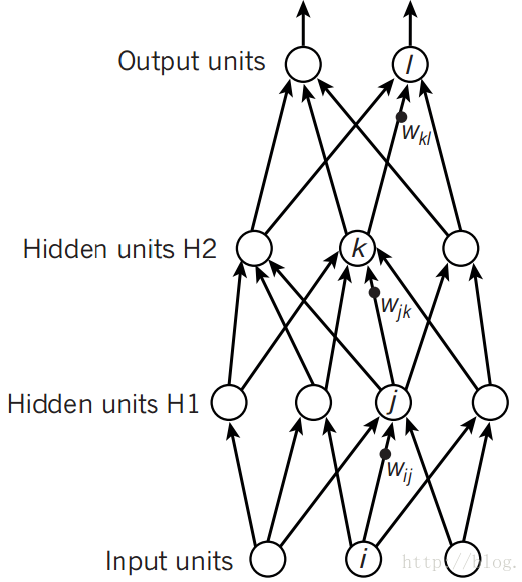
\includegraphics[scale=0.25]{20171216112534046.png}
    			\caption{全连接神经网络示意图\protect\footnotemark[1]}
    			\label{neuralNetWork}
    		\end{figure}
    		\footnotetext[1]{图片来自网络}
            
    		\indent 所谓前向传播,其实就是计算一个十分复杂的复合函数。图\ref{neuralNetWork}中每一个节点都代表着两次计算:
    		\begin{align}
    			&{z}^{[l]}={w}^{[l]}\cdot{a}^{[l-1]}+{b}^{[l]} \label{forw:z} \\
    			&{{a}^{[l]}}={{\sigma}^{[l]}}\left({{z}^{[l]}}\right) \label{forw:a}
    		\end{align}
    		其中$\sigma(x)=\frac{1}{1+e^{-x}}$,我们称其为“激活函数”。
    		
    		\indent 从这里我们可以看出,从输入节点开始,沿任意路径到一个输出节点,就构成了一个复合函数,且每一层函数都有着相同的形式。同时我们也可以看出,这若干个复合函数在一起就构成了一个神经网络。
    		
    	\subsection{反向传播}\label{backward}
    		
    		\indent 不难想见,若不加任何处理,随机设置公式\ref{forw:a}中的参数$w$和$b$的值,得到的结果肯定也是随机的,我们无法用其来进行任何决策或预估。所以我们需要减少误差,而要减小误差我们必须要有真值才行,于是这里又涉及到有监督学习与梯度下降法的问题,我们将分别在\ref{datasets}节和\ref{梯度下降法}节讲述。
    		
    		
    		\subsubsection{数据集与有监督学习}\label{datasets}
    			\indent 深度学习得以进行的一大前提条件就是数据集。我们通过给模型大量的数据进行训练使其能够完成特定的任务。
    			
    			\indent 数据集通常会分为训练集和测试集,训练集和测试集中又会被分为样本和真值两个部分。而对样本或真值的处理就分出了有监督和无监督学习。
    						
    			\indent 有监督学习,顾名思义,就是需要人为的“监控”。这里所说的“监控”其实就是指为每一个训练样本和测试样本标注真值,或者是对输入样本进行一些手工处理。
    			
    			\indent 相应的,如果不对数据做任何处理,则称为无监督学习。
    			
    		\subsubsection{梯度下降法}\label{梯度下降法}
    			\indent 关于梯度下降法的作用我们可以形象地理解为“找谷底”,如图\ref{gradient_descent}所示。
    			
    			\begin{figure}[H]
                    \centering
        			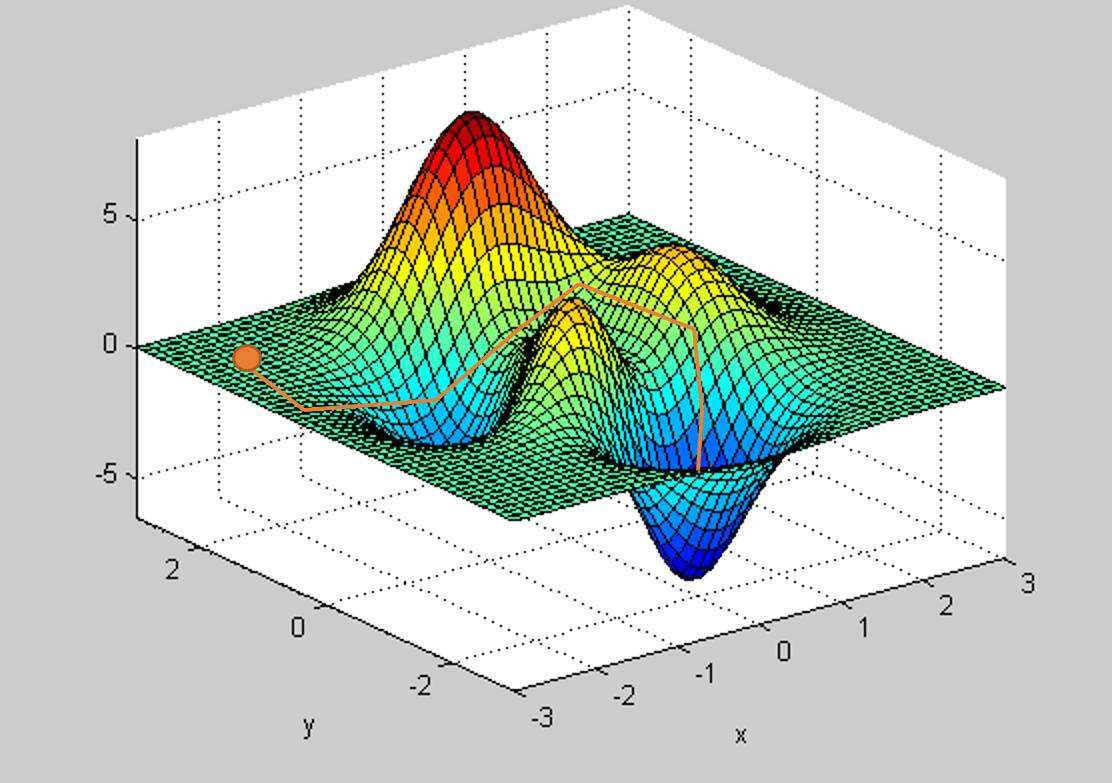
\includegraphics[scale=0.3]{gradient_descent.jpeg}
        			\caption{梯度下降示例\protect\footnotemark[1]}
        			\label{gradient_descent}
    		    \end{figure}
    			\footnotetext[1]{图片来自网络}
                
    			\indent 假设我们现在正处在一个山谷的某处,需要走到谷底,但却不知道路线,怎么办?这种情况下一种理论上可行的办法是朝着当前位置最陡峭的方向向下迈一步,之后再向新位置最陡峭的方向向下迈一步,如此反复,不出意外的话,我们肯定可以到达谷底。
    			
    			\indent 上述过程其实就是梯度下降法的原理。现在我们有了一个很大很深的神经网络,可以通过前向传播算出一个结果,同时对于每一个输入都有一个真值与之对应,所以接下来要做的就是如何利用这些条件来找出输入与输出之间的对应关系。
    			
    			\indent 在第\ref{forward}节中曾说过,一个神经网络其实就是若干个复合函数并列放在一起,并且只要这些复合函数足够“复杂”,我们就可以用这个神经网络来拟合数据集中输入与输出的关系。但如果仅仅去随机初始化网络中的参数,很难得到一个令人满意的结果,所以在初始化之后我们还需要去优化这些参数,使得神经网络输出的结果尽可能接近真值。所用的方法就是梯度下降。
    			
    			\indent 对于一个多元函数,我们想要求它的极小值,常用的做法是求它的导函数,令其等于0。然而这种做法难以编程实现,因而可以借鉴上述“找山谷”的思路:先求出当前点的梯度,然后令坐标向梯度的负方向移动一小步,之后再求新位置的梯度,并重复之前的步骤,这样就可以逐渐移至极小值点附近。而在深度学习中,我们就是用这样的方式优化每一个节点中的参数值,最终使得整个网络可以较好地去拟合输入输出之间的关系。
    			
%    			\indent 值得一提的是,我们不太关心神经网络拟合出的关系具体是怎样的。虽然每一个节点的函数形式都是固定的,我们也完全可以把它们的参数全部输出出来,但几乎没有人会这么做。因为一方面,一个神经网络的参数非常多,有时可能达到上十亿个,想要把若干个拥有如此多参数的复合函数写出来基本是不可能的;另一方面,在实际应用中也无须知道这些复合函数究竟是什么样的,我们只用将训练好的神经网络的结构与参数保存下来,在使用时将其导入即可。
    			
    		\subsubsection{反向传播的具体实现}
    			\indent 有了梯度下降的概念后,我们就不难想出具体的实现方法,也就是反向传播。
    			
    			\indent 由于每一个节点的函数形式都是固定的,那么它的导函数形式也是固定的,根据式\ref{forw:z}和式\ref{forw:a}我们可以很容易写出(公式中的$J$表示神经网络最终的输出):
    			\begin{align}
    			&\frac{\partial J}{ \partial {{z}^{[l]}} }=\frac{\partial J}{\partial {{a}^{[l]}}}*{{\sigma}^{[l]}}'( {{z}^{[l]}})  \\
    			&\frac{\partial J}{\partial {{w}^{[l]}}}=\frac{\partial J}{\partial {{z}^{[l]}}}\cdot{{a}^{[l-1]}} \\
    			&\frac{\partial J}{\partial {{b}^{[l]}}}=\frac{\partial J}{\partial {{z}^{[l]}}} \\
    			&\frac{\partial J}{\partial {{a}^{[l-1]}}}= \frac{\partial J}{\partial {{z}^{[l]}}} \cdot {{w}^{\left[ l \right]}}
    		    \end{align}
    			
    			\indent 在优化时,我们令:
    			\begin{align}
    			&w^{[l]}=w^{[l]}-\alpha \cdot \frac{\partial J}{\partial {{w}^{[l]}}} \\
    			&b^{[l]}=b^{[l]}-\alpha \cdot \frac{\partial J}{\partial {{b}^{[l]}}}
    			\end{align}
    			这里$\alpha$叫学习率,相当于我们在\ref{gradient_descent}节中说的所跨一步的步长,是一个需要人根据经验来调节的超参数。
                
    \section{卷积神经网络}\label{cnn}
        
        \indent 在介绍完了深度学习工作的基本过程之后,再来讲述卷积神经网络的基本原理就要容易得多了。同样,我们将分三个小节来对其进行描述。
        
        \subsection{全连接网络的缺陷}
        
            \indent 在\ref{forward}节中我们曾给出了全连接神经网络的示意图。然而在现实情况中,比如处理一张图片时,这样做会产生巨大的运算量。例如我们要处理一张$1024\times1024$的图片,那么仅仅在输入层就会有超过$100$万个节点,这样势必会产生大量的开销。另外,由于在输入图像时,会将一张图片“拉”成一个向量,这样在一定程度上还会损失结构信息。
            
        \subsection{卷积神经网络的优势及工作过程}\label{process_of_cnn}
        
            \indent 为了应对上述情况,人们提出了卷积神经网络,通过对卷积核的复用来减少网络参数。这里的卷积核其实就相当于一个滤波器,逐步扫描整幅图像,把卷积核中的各点值与对应的图片像素相乘再相加,得到的结果放在卷积核中心对应的图像位置上,如图\ref{convolution}所示。
            
            			\begin{figure}[H]
            				\centering 
            				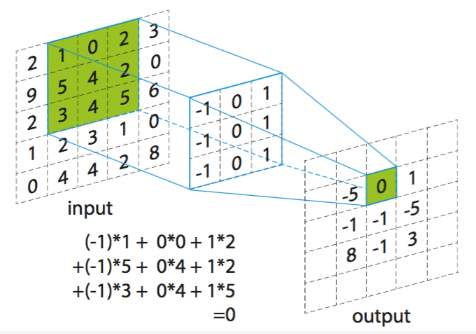
\includegraphics[scale=0.7]{convolution.jpg} 
            				\caption{卷积核的工作过程\protect\footnotemark[1]} 
            				\label{convolution}
            			\end{figure}
                        \footnotetext[1]{图片来自网络}
            
            \indent 在这种情况下,网络需要学习的参数就变成了卷积核(或者说滤波器)每个点的值。但由于每一层的卷积核数量往往不会太多,所以需要学习的参数也会大大减少。
            
        \subsection{卷积神经网络的基本思想}
            
            \indent 到这里我们可能会有些疑问:为何每一层的卷积核数量不用太多?
            
            \indent 其实正如\ref{process_of_cnn}节所说的,每一个卷积核可以被理解为一个滤波器,而滤波器的功能就是提取图像中的某一类信息,且能够被同一个滤波器提取出来的信息都具有某种相同的“模式”。\textbf{更确切地说,图像中具有某种相同模式的信息都能够被同一个滤波器提取出来},例如变化剧烈的边缘可以用拉普拉斯算子等提取,而这也正是卷积核数量不用太多的原因!
            
            \indent 从直观感受来看,不论图像有多复杂,都能够被看作是由一系列基本的要素构成的,而这些要素正是图案的模式。比如一个图像的轮廓可以看作是由若干条不同角度的小线段组成,所以为了提取它的轮廓,我们可以用对应数量的滤波器来进行卷积,每一种滤波器都专门用来提取某个特定的要素。更关键的是,\textbf{在某一个局部图案中可以找到的要素,往往也能在其它图案总找到},比如桌子和课本都有可能会包含垂直的小线段。
            
            \indent 基于这样的假设,我们就可以用少量的滤波器,即卷积核,来提取一整幅图像中所有需要的信息,从而达到减少参数的目的。而从实际应用的效果来看,该假设是完全成立的。
    			
    \section{深度学习中的一些问题}
        		\indent 第\ref{deeplearning}节和第\ref{cnn}节介绍了深度学习及卷积神经网络的工作方式及基本原理,本节我们将讨论深度学习中存在的部分问题作为补充。
        		\subsection{梯度消失与梯度爆炸}
        		\indent 我们在第\ref{forward}节中曾提到过激活函数$\sigma(x)$,同时在第\ref{backward}中不难看出在优化网络参数时无法回避对激活函数求导,那么我们现在来考察一下$\sigma(x)$导函数的性质:	
        		\begin{equation}
        		\begin{split}
        		\sigma'(x) &= \frac{e^{-x}}{(1+e^{-x})^2} \\
        		&= \frac{1}{1+e^{-x}} - \frac{1}{(1+e^{-x})^2} \\
        		&= \sigma(x) - [\sigma(x)]^2 \\
        		&\leq \frac{1}{4}
        		\end{split} 
        		\end{equation}		
        		\indent 由于我们在进行梯度反传时实际上是在用链式法则求导数,所以随着层数的加深,导数的数值会以指数形式下降,这就导致了反向传播越往前,效果越微弱,致使前后层训练的步调不一致,尤其是靠近输入层的参数,几乎无法得到优化。
        		
        		\indent 相应的,如果激活函数的导数大于1,则在反向传播中导数值会以指数形式上升,造成梯度爆炸。不过这种情况很少见。
        		
        		\indent 这个问题到现在应该说还没有彻底解决,但经过前人的努力,也有了许多不错的方案。其中一个效果比较好的是用其它激活函数来替代$\sigma(x)$,而在所有替代品中,$relu$函数脱颖而出,有效地缓解了梯度消失,并得到广泛认可。它的表达式如下:	
        		\begin{equation}
        			\begin{split}
        				relu(x) = max(0, x)
        			\end{split}	
        		\end{equation}
        		
        		\subsection{局部极值点}
        		\indent 从图\ref{gradient_descent}中我们可以看出,一个函数很可能有多个极值点,但实际需要的只有一个全局的最值点。然而,梯度下降法只能让我们找到某一个极值点,却无法判断这个点是否为全局最优。
        		
        		\indent 针对这个问题也有许多解决方式被提出,不过很难说哪种方式可以彻底解决它。一种常见做法是用不同的权重来初始化整个网络,尤其是用别人已经在某些相近数据集上训练好的参数。这样做可以使得我们有较大的概率将整个网络参数初始化在最优点附近,从而避免落入其它局部极值点。
    		
    		
%    		\section{深度学习现状及发展}
%    		\indent 读过本文后,相信大家肯定还有很多疑惑。一方面受笔者水平、时间所限,很难在这短短数千字内将深度学习的原理彻底讲清楚;另一方面,关于深度学习基础的数学研究,实际上还处在非常初级的阶段,很多研究成果都是依据研究者的经验以及大量实验做出来的,但为何这么做,很多时候其实研究者自己也讲不清除。
%    		
%    		\indent 以MUNIT\cite{huang2018munit}为例,其整篇论文都是基于作者的若干个猜想建立起来的,再配以大量试验结果来证明自己方法的优越性,却始终给不出严格的推导证明。事实上,能够像GAN\cite{Goodfellow2014Generative}那样在提出一个崭新的算法后又能给出理论上严格证明的还是少数。
%    		
%    		\indent 在我看来,现在科研人员们对深度学习的推广就如同18世纪数学家们对微积分的推广。很多时候我们其实并不清楚到底发生了什么,可效果就是变好了,就连在人工智能领域赫赫有名的吴恩达也不得不承认这一点。而由于缺乏理论的支持,很多参数的调整以及网络结构的优化等许多任务都是依靠人的经验和直觉才做成的,且这些经验很难在各个领域之间移植。
%    		
%    		\indent 尽管这样的状况大概还会持续相当长一段时间,但令人欣喜的是,对于深度学习的理论研究也有人在不断推进。我们有理由相信,深度学习和人工智能仍会飞速发展,并为人类、为社会带来越来越多的惊喜。
%			
%			\begin{enumerate}[leftmargin=50pt]
%				\item 由条带传感器成像,给出一幅图像一行(或一列)的像素值;
%				\item 沿垂直于传感器带的方向移动一小段距离;
%				\item 重复步骤$1$和步骤$2$,直至整幅图像全部成像完毕。
%			\end{enumerate}

		

	\section{总结:一点个人理解}
	   \indent 通过梳理神经网络的相关知识,个人感觉深度学习(主要是有监督学习)更多地是一个极大似然估计的过程。所谓极大似然估计,就是在已知实验结果的情况下,反推最有可能导致这种结果的所有参数。换句话说,就是要找出最优参数,使得似然函数输出的结果能够最大程度接近已知的结果。而梯度下降法所做的,正是这样的事情:不断优化参数,使得网络的输出尽可能接近标记的值。所以在我看来,所谓深度学习,就是极大似然估计的一种实现;而深度神经网络,其实就是一个及其复杂的似然函数。
		
%			\begin{figure}[H]
%				\centering 
%				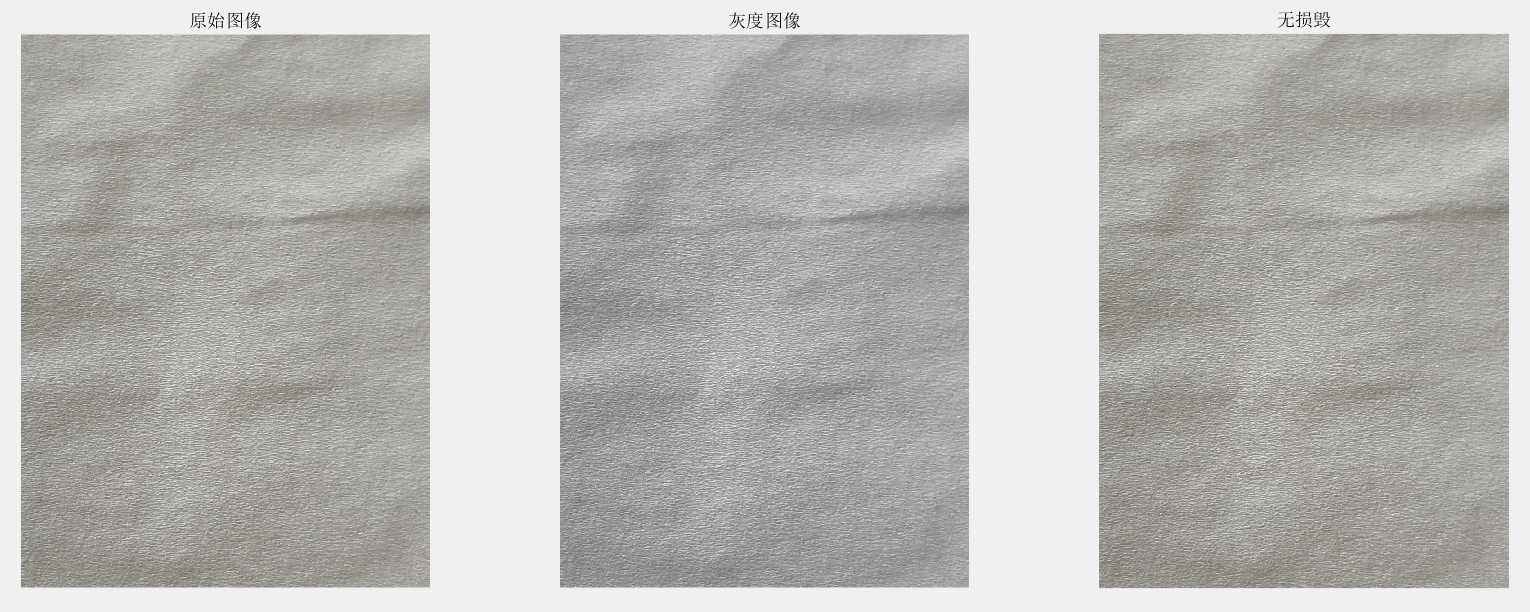
\includegraphics[scale=0.4]{res4.png} 
%				\caption{结果4} 
%				\label{res4}
%			\end{figure}
		

		
%			\begin{figure}[H]
%				\centering 
%				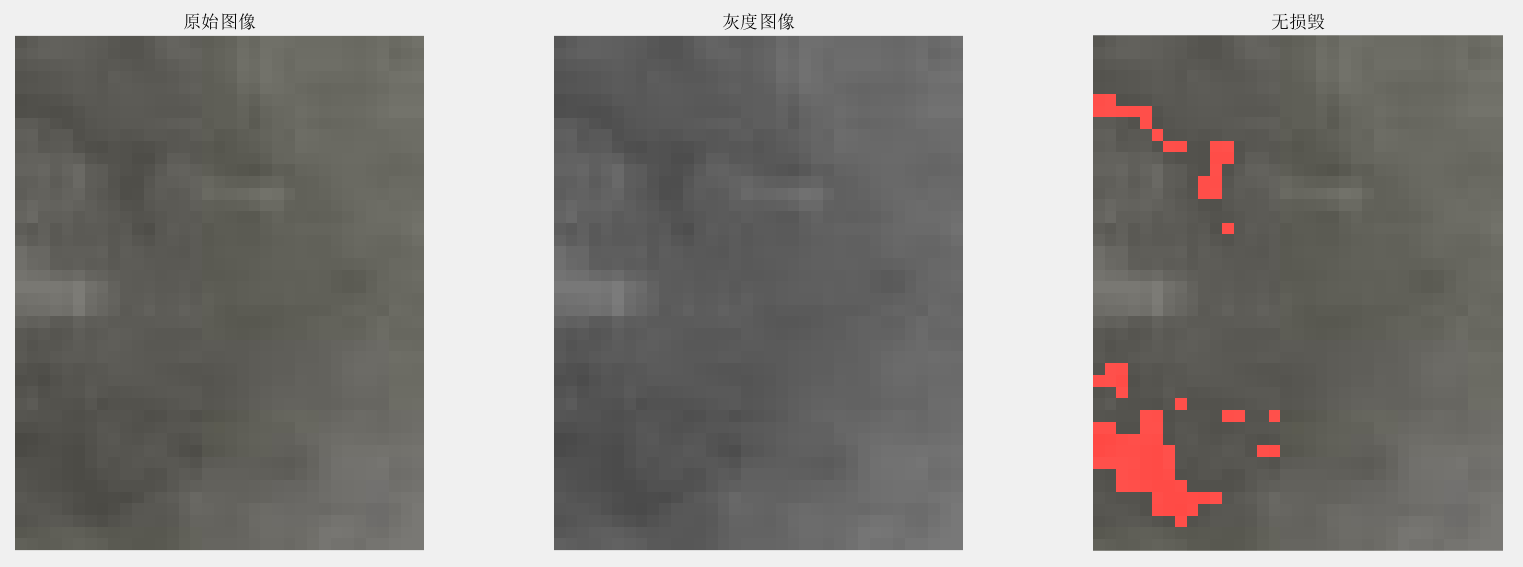
\includegraphics[scale=0.4]{res6.png} 
%				\caption{结果6(截取自结果5的阴影部分)} 
%				\label{res6}
%			\end{figure}
	
	
% 中文文献多个作者用中文逗号“,”连接
%\bibliography{ref.bib}
%\bibliographystyle{abbrv}
\bibliography{ref.bib}


\end{document}